\documentclass[11pt,a4paper,ngerman]{article}

\usepackage[table]{xcolor}
\usepackage{autotuwien}
\usepackage{tabularx}
\usepackage{ragged2e}
\usepackage{multirow}

\usepackage[printwatermark]{xwatermark}
\newwatermark[allpages,color=red!10,angle=45,scale=6,xpos=-1cm,ypos=1cm]{DRAFT}


% left justify footnotes
\usepackage[flushmargin,hang]{footmisc}
\renewcommand{\footnotelayout}{\raggedright}


\lecture{ITIA}
\semester{Dokumentation}
\title {Targetbeschreibung}
\author{Dieter Etz \\ {\small \href{mailto:dieter.etz@tuwien.ac.at}{dieter.etz@tuwien.ac.at}}}
\date{\today}

\makeatletter
 \let\mytitle\@title
 \let\myauthor\@author
 \let\mysubject\@lecture
\makeatother
\hypersetup{%
pdfauthor={\myauthor},
pdftitle={\mytitle},
pdfsubject = {\mysubject}
}


\begin{document}
\maketitle
\tableofcontents
%\abstract{}   
\newpage

\section{Zielsetzung}

Die vorliegende Beschreibung enthält die für die Lösung der Beispiele wesentlichen Informationen über Aufbau und Funktionsweise der Targetsysteme.


\section{Übersicht}

Das Gesamtsystem besteht aus 4 Targets, jedes Target besteht aus einer bzw. zwei Stationen.
\begin{center}
	%\rowcolors{2}{white}{gray!25}
	\setlength\extrarowheight{4pt}
	\small
	\begin{tabular}{|p{4cm}|p{4cm}|}
		\rowcolor{gray!80}
		\hline
		\bf Target  & \bf Station\\
		\hline\hline
		\multirow{2}{*}{Target 12} & Station 1: Verteilen\\
		 & Station 2: Prüfen\\
		\hline
		\multirow{2}{*}{Target 34} & Station 3: Bearbeiten\\
		& Station 4: Handhaben\\
		\hline
		\multirow{2}{*}{Target 56} & Station 5: Puffern\\
		& Station 6: Sortieren\\
		\hline
		Target Rob & Station Rob\\
		\hline
	\end{tabular}
\end{center}

Der Ablauf und Materialfluss sind in Abbildung \ref{fig_system_structure} dargestellt.

\begin{figure}[!htb]
	\centering
	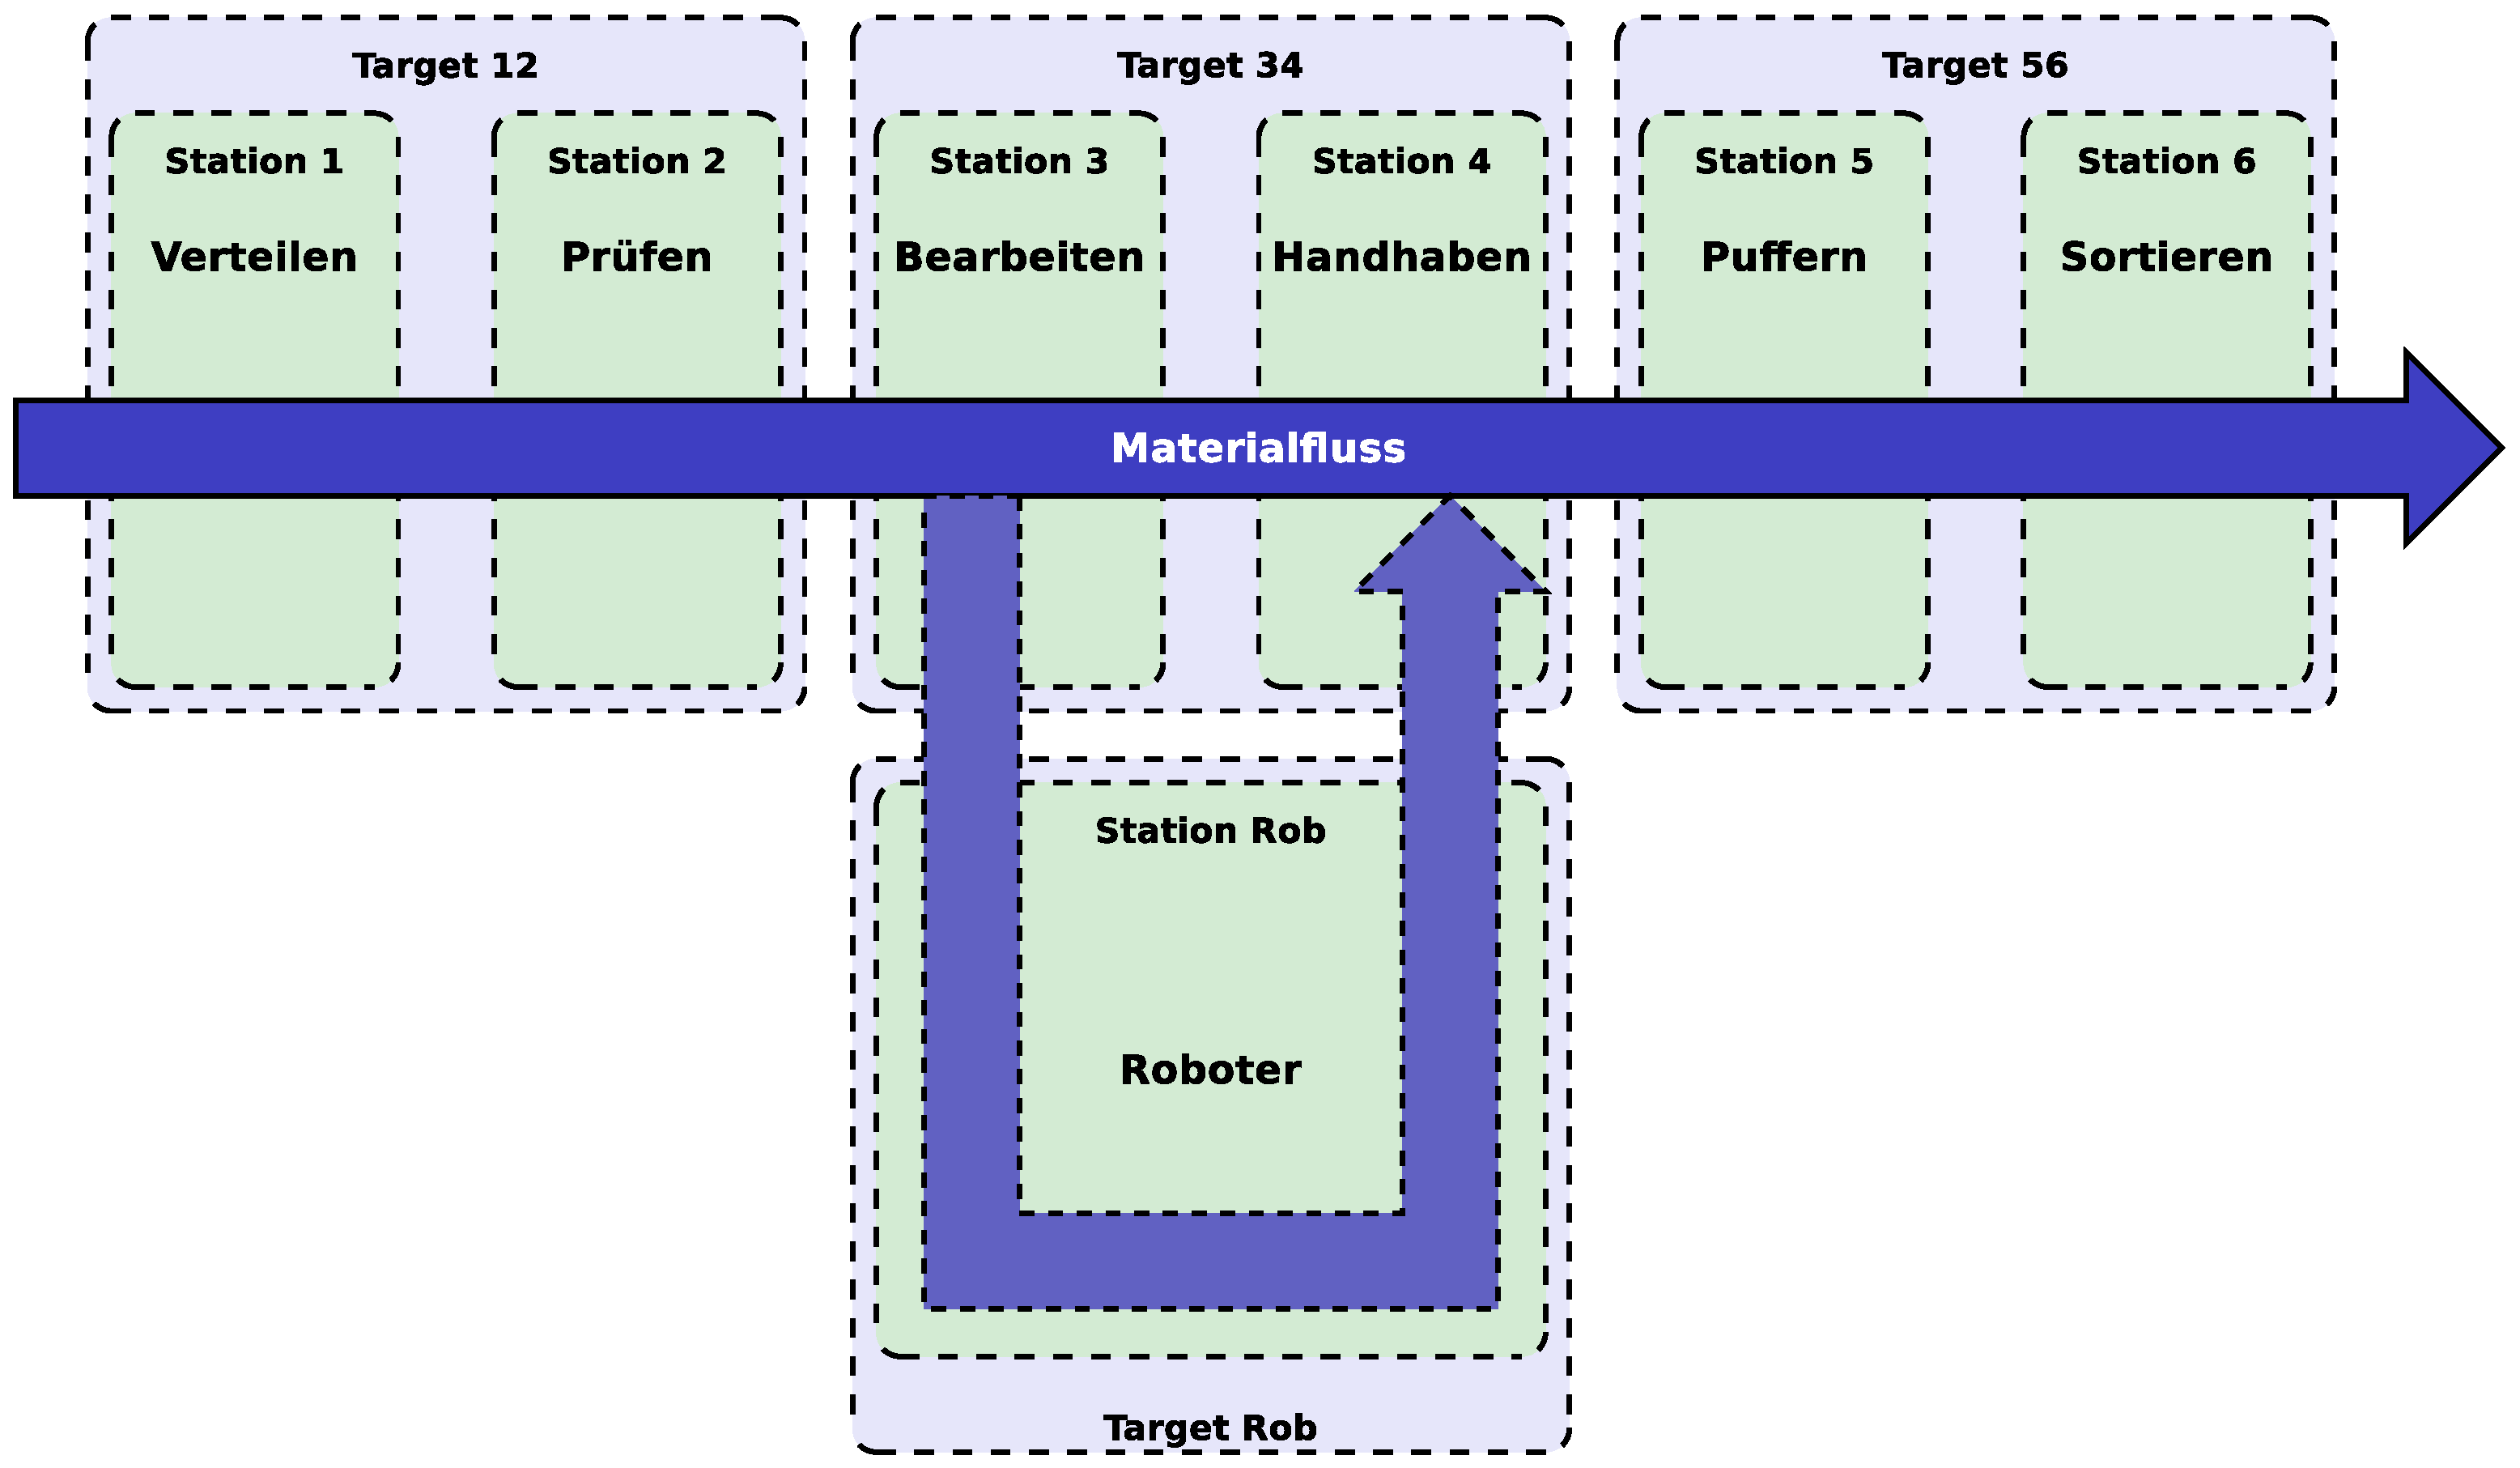
\includegraphics[width=.99\linewidth]{images/System_Structure}
	\caption{Gesamtsystem Struktur}
	\label{fig_system_structure}
\end{figure}

Jedes Target verfügt über ein programmierbares Steuerungssystem. Bei Target 12, Target 34, und Target 56 ist dies eine industrielle SPS. Am Target Rob befindet sich ein programmierberer Roboter Controller.


\section{Aufbau Target 12}

\subsection{Station 1: Verteilen}\label{station_verteilen}
Das Modul Verteilen reicht die Werkstücke an die Station 2 „Prüfen“ weiter.

\subsubsection{Module}

\paragraph{Stapelmagazin}
Das Stapelmagazin enthält die zu bearbeitenden Werkstücke, vereinzelt diese und bietet dabei Platz für 10 Werkstücke. Mithilfe eines optischen Sensors kann gemessen werden, ob das Magazin leer ist oder Werkstücke enthält. Mittels eines doppeltwirkenden Zylinders kann das unterste Werkstück aus dem Fallmagazin heraus geschoben werden. Das Magazin kann mit Werkstücken beliebiger Farbe aus beliebigem Material befüllt werden. Es ist zu beachten, dass diese, in der Reihenfolge in der sie im Magazin liegen, von unten nach oben der Reihe nach abgearbeitet werden. Das Magazin ist also eine Art FIFO-Buffer.

\paragraph{Umsetzen}
Der Umsetzer ist ein pneumatisches Handlinggerät und besteht aus einem Greifarm und einen Vakuumsauger. Der Greifarm ist als pneumatischer Schwenkantrieb realisiert und kann zwischen 0° bis 180° geschwenkt werden. Der Schwenkantrieb hat eine Endlagenabfrage, kann aber auch Positionen zwischen 0° und 180° anfahren. Der Vakuumsauger hat die Aufgabe, das Werkstück wärend des gesamten Schwenkvorganges anzusaugen und so zu transportieren.


\subsubsection{Sensoren/Aktoren}


\begin{center}
  \rowcolors{2}{white}{gray!25}
  \setlength\extrarowheight{4pt}
  \small
  \begin{tabularx}{\textwidth}{|p{4cm}|X|}
  	\hline
  	\rowcolor{tublau}
  	\multicolumn{2}{|c|}{\bf \color{white} \large Sensoren}\\
  	\hline\hline
    \rowcolor{gray!80}
    \bf Name & \bf Beschreibung\\
    \hline\hline
    S1\_Cylinder\_IsIn &  Vereinzelungszylinder-Endschalter hinten = 1, wenn Vereinzelungszylinder hinten ist.\\
    S1\_Magazine\_IsEmpty & optischer Näherungsschalter = 1, wenn das Magazin leer ist.\\
    S1\_Swivel\_IsLeft & Schwenkarm in linker Endposition.\\
    S1\_Swivel\_IsRight & Schwenkarm in rechter Endposition.\\
    S1\_Item\_IsPresent & Werkstück befindet sich am Sauger.\\
    S1\_Button[0..3] & 4 farbige Taster.\\
    \hline
  \end{tabularx}

  \medskip
  
  \begin{tabularx}{\textwidth}{|p{4cm}|X|}
  	\hline
  	\rowcolor{tublau}
  	\multicolumn{2}{|c|}{\bf \color{white} \large Aktoren}\\
  	\hline\hline
    \rowcolor{gray!80}
    \bf Name & \bf Beschreibung\\
    \hline\hline
    S1\_Cylinder\_Eject & Nächstes Werkstück aus dem Magazin entnehmen. (Einfachwirkend).\\
    S1\_Vacuum\_On & Werkstück ansaugen.\\
    S1\_Vacuum\_Off & Werkstück loslassen.\\
    S1\_Swivel\_Left & Schwenkarm nach links bewegen.\\
    S1\_Swivel\_Right & Schwenkarm nach rechts bewegen.\\
    S1\_Lamp[0..3] & Lampen für die Taster.\\
    \hline
  \end{tabularx}
\end{center}

\begin{itemize}
	\item[\bf Hinweis:] S1\_Cylinder\_Eject darf nur aktiviert werden wenn sich der Schwenkarm nicht in der linken Endposition befindet. Der Sauger könnte dadurch beschädigt werden.
\end{itemize}

\begin{itemize}
	\item[\bf Hinweis:] S1\_Swivel\_Right darf nur aktiviert werden wenn sich der Lift in der unteren Endposition befindet und sich kein Werkstück am Lift befindet.
\end{itemize}



\subsection{Station 2: Prüfen}\label{station_pruefen}

\subsubsection{Module}

Die Station kann in vier Module eingeteilt werden, die jeweils die Hauptaufgaben dieser Station widerspiegeln: Erkennen, Messen, Transport (Heben und Schieben), Weitergeben (Rutsche).

\paragraph{Erkennen}
Dieses Modul beinhaltet 3 Näherungsschalter: kapazitiv, induktiv und optisch. Damit lassen sich Werkstücke in die Kategorien „Rot“, „Metall“, „Kunststoff“ einteilen. In diesem Schritt können schon die ersten ungültigen Teile ausgeworfen werden (mittels Ausschiebezylinder, siehe Modul Heben und Schieben). Die folgende Tabelle gibt an, welcher Sensor bei welcher Art von Werkstück anspricht.

\begin{center}
  \rowcolors{2}{white}{gray!25}
  \setlength\extrarowheight{4pt}
  \small
  \begin{tabular}{|p{5cm}|>{\Centering}p{1.5cm}|>{\Centering}p{1.5cm}|>{\Centering}p{1.5cm}|}
    \rowcolor{gray!80}
    \hline
    \bf  & \bf induktiv & \bf kapazitiv & \bf optisch \\
    \hline\hline
    Werkstück vorhanden & & X & \\
    Metall & X & X & X \\
    Kunststoff & & X & \\
    rot & & X & X \\
    \hline
  \end{tabular}
\end{center}

Aufgrund der Eigenschaften der Sensoren werden folgende Verknüpfungen angewandt, um ein Werkstück zu klassifizieren (jeweils 1 Bit pro Klasse):
\begin{itemize}
\item Werkstück vorhanden $:= sensor\_kap$
\item Werkstück aus Metall $:= sensor\_ind$
\item Werkstück ist rot $:= sensor\_opt \land \lnot sensor\_ind$
\end{itemize}

Der kapazitive Sensor spielt eine große Rolle beim Implementieren der Funktionen dieser Station. Er bewegt sich mit dem Werkstück auf dem Modul Heben und Schieben im Gegensatz zu den anderen beiden Sensoren und kann somit zum Steuern des Ausschiebezylinders verwendet werden oder den eigentlichen Betrieb (Erkennen, Messen, Heben, Weitergeben) einleiten.

\paragraph{Heben und Schieben}
Dieses Modul kann das Werkstück auf- und abbewegen. Um ein neues Werkstück (von der Station Verteilen) zu erhalten, muss die Förderanlage in den Grundzustand „unten“ gebracht werden. Nach dem Erkennen des Werkstücks (siehe Modul Erkennen) wird das Werkstück mit einem Ausschiebezylinder ausgeworfen oder nach oben befördert. Am Anschlag der Hebevorrichtung kann die Höhe des Werkstücks kontrolliert (siehe Module Messen) und das Werkstück an das Modul Rutsche weitergereicht werden.

\paragraph{Messen}
Dieses Modul enthält einen analogen Sensor, der die Werkstückshöhe angibt. Falls die Höhe einen bestimmten Wert über- bzw. unterschreitet, muss das Werkstück mit dem Modul Heben und Schieben wieder zum Auswurf (am unteren Ende der Hebevorrichtung) befördert werden.

\paragraph{Rutsche}
Ist das Werkstück gültig (d.h., alle Kontrollen - Farbe, Material, Höhe - bestanden), wird es vom Ausschiebezylinder am Modul Heben und Schieben auf die Rutsche befördert. Die Rutsche ist leicht geneigt. Ein Stopper kann das Werkstück davor bewahren, zu einem ungünstigen Zeitpunkt zur nächsten Station zu wechseln. D.h., wenn die Station Bearbeiten für die Übergabe noch nicht bereit ist, kann der Stopper aktiviert werden. Sobald die nächste Station das OK gibt, soll der Stopper eingefahren werden und so das Werkstück weitergeben.


\subsubsection{Sensoren/Aktoren}
\begin{center}
	\rowcolors{2}{white}{gray!25}
	\setlength\extrarowheight{4pt}
	\small
	\begin{tabularx}{\textwidth}{|p{4cm}|X|}
		\hline
		\rowcolor{tublau}
		\multicolumn{2}{|c|}{\bf \color{white} \large Sensoren}\\
		\hline\hline
		\rowcolor{gray!80}
		\bf Name & \bf Beschreibung\\
		\hline\hline
		S2\_Sensor\_Ind & induktiver Näherungsschalter = '1', wenn ein metallisches Werkstück vorhanden ist.\\
		S2\_Sensor\_Cap & kapazitiver Näherungsschalter = '1', wenn ein Werkstück vorhanden ist.\\
		S2\_Sensor\_Opt & optischer Näherungsschalter = '1', wenn ein rotes oder metallisches Werkstück vorhanden ist.\\
		S2\_Raiser\_IsBot & Heben-Endschalter unten = '1', wenn sich die Hebevorrichtung in der Ausgangsposition „unten“ befindet.\\
		S2\_Raiser\_IsTop & Heben-Endschalter oben = '1', wenn sich die Hebevorrichtung am oberen Anschlag befindet.\\
		S2\_Pusher\_IsIn & Ausschieber-Endschalter = '1', wenn der Ausschiebezylinder eingefahren ist.\\
		S2\_Measure\_Height & Linearpotentiometer zum Messen der Werkstückhöhe, der Wertebereicht liegt bei 16\#0008..6C6C (8..27756).\\
		S2\_Measure\_IsReady & Linearpoti ist in Position gebracht (heruntergefahren) = '1', sonst '0'.\\
		S2\_Button[0..3] & 4 farbige Taster = '1', wenn er gedrückt ist.\\
		\hline
	\end{tabularx}
	
	\medskip
	
	\begin{tabularx}{\textwidth}{|p{4cm}|X|}
		\hline
		\rowcolor{tublau}
		\multicolumn{2}{|c|}{\bf \color{white} \large Aktoren}\\
		\hline\hline
		\rowcolor{gray!80}
		\bf Name & \bf Beschreibung\\
		\hline\hline
		S2\_Raiser\_Up & Hebevorrichtung nach oben fahren; Mit '1' wird die Hebevorrichtung nach oben gefahren. Wenn '0' anliegt steht sie still.\\
		S2\_Raiser\_Down & Hebevorrichtung nach unten fahren; Mit '1' wird die Hebevorrichtung nach unten gefahren. Wenn '0' anliegt steht sie still.\\
		S2\_Measure\_Act & Linearpoti zum Messen der Höhe nach unten fahren; Um nach unten zu fahren, sollte '1' solange angelegt werden, bis S2\_Measure\_IsReady '1' wird und S2\_Measure\_Height gemessen wurde. Wenn anschließend '0' angelegt wird, fährt das Gerät selbstständig in die Ausgangsposition.\\
		S2\_Push\_Act & Ausschiebezylinder ausfahren; Solange dieser Ausgang auf '1' gesetzt wird, bewegt sich der Zylinder nach außen. Sobald der Wert auf '0' springt, wird der Zylinder eingezogen.\\
		S2\_Stopper\_Act & Stopper ausfahren; Dieser wird mit '1' blitzartig ausgefahren, sobald der Wert '0' ist wieder eingefahren (Rutsche freigegeben).\\
		S2\_Lamp[0..3] & 4 farbige Lampen für die Taster; Die Lampen leuchten bei '1'.\\
		\hline
	\end{tabularx}
\end{center}

\begin{itemize}
	\item[\bf Hinweis:] S2\_Raiser\_Up und S2\_Raiser\_Down dürfen nur aktiviert werden wenn sich der Schwenkarm nicht in der rechten Endposition befindet.
\end{itemize}


\subsection{SPS Komponenten}

\begin{center}
	%\scriptsize
	\setlength\extrarowheight{2pt}
	\begin{tabular}[t]{p{8cm}l}
		\rowcolors{2}{gray!25}{white}
		\begin{tabular}[t]{|p{1.2cm}p{4.5cm}|}
			\hline
			\rowcolor{gray} \multicolumn{2}{|c|}{\bf SPS}\\
			\hline\hline
			Device: & CPU 1513-1 PN\\
			ID: & 6ES7 513-1AL02-0AB0\\
			MAC: & ac:64:17:57:b1:0b\\
			IP: & 192.168.162.33/25\\
			\hline
		\end{tabular}
	
		\vspace{5mm}
		
		\begin{tabular}[t]{|p{1.2cm}p{4.5cm}|}
			\hline
			\rowcolor{gray} \multicolumn{2}{|c|}{\bf HMI}\\
			\hline\hline
			Device: & TP1500 Comfort V2\\
			ID: & 6AV2 124-0QC02-0AX1\\
			MAC: & ac:64:17:55:1e:42\\
			IP: & 192.168.162.37/25\\
			\hline
		\end{tabular} &
	
		\rowcolors{2}{gray!25}{white}
		\begin{tabular}[t]{|p{1.2cm}p{5.5cm}|}
			\hline
			\rowcolor{gray} \multicolumn{2}{|c|}{\bf IO Device}\\
			\hline\hline
			Device: & IM155-6 PN HF\\
			ID: & 6ES7 155-6AU01-0CN0\\
			MAC: & ac:64:17:80:57:4a\\
			IP: & 192.168.162.34/25\\
			& \vspace{-5pt}\small\rowcolors{2}{gray!25}{white}
			\begin{tabular}{|p{0.4cm}p{4.4cm}|}
				\hline
				\rowcolor{gray!80}
				Slot & Modul \\
				\hline\hline
				1 & \parbox{4cm}{\vspace{2pt}\tiny CM AS-i Master ST\\3RK7 137-65A00-0BC1\vspace{2pt}}\\[2pt]
				2 & \parbox{4cm}{\vspace{2pt}\tiny DI 8x24VDC HF\\6ES7 131-6BF00-0CA0\vspace{2pt}} \\
				3 & \parbox{4cm}{\vspace{2pt}\tiny DI 8x24VDC HF\\6ES7 131-6BF00-0CA0\vspace{2pt}} \\
				4 & \parbox{4cm}{\vspace{2pt}\tiny AI 4xU/I 2-wire ST\\6ES7 134-6HD01-0BA1\vspace{2pt}} \\
				5 & \parbox{4cm}{\vspace{2pt}\tiny DQ 8x24VDC/0.5A HF\\6ES7 132-6BF00-0CA0\vspace{2pt}} \\
				6 & \parbox{4cm}{\vspace{2pt}\tiny DQ 8x24VDC/0.5A HF\\6ES7 132-6BF00-0CA0\vspace{2pt}} \\
				\hline
			\end{tabular}
			\vspace{-1pt}	
			\\
			\hline
		\end{tabular} \\
	\end{tabular}
\end{center}


\begin{center}
	\rowcolors{2}{white}{gray!25}
	\setlength\extrarowheight{4pt}
	\small
	\begin{tabularx}{\textwidth}{|p{1.5cm}|p{1cm}|p{4cm}|X|}
		\hline
		\rowcolor{tublau}
		\multicolumn{4}{|c|}{\bf \color{white} \large Eingänge}\\
		\hline\hline
		\rowcolor{gray!80}
		\bf Adresse & \bf Label & \bf Name & \bf Beschreibung \\
		\hline\hline
		E0.0  &     & S1\_ButtonY & Taster gelb.\\
		E0.1  &     & S1\_ButtonG & Taster grün.\\
		E0.2  &     & S1\_ButtonW & Taster weiß.\\
		E0.3  &     & S1\_ButtonR & Taster rot.\\
		E32.0 & B4  & S1\_Magazine\_IsEmpty & Magazin ist leer.\\
		E32.1 & 1B2 & S1\_Cylinder\_IsIn & Ausfurfzylinder ist in der hinteren Position.\\
		E32.2 & 3S2 & S1\_Swivel\_IsLeft & Umsetzer in der linken Position.\\
		E33.2 & 3S1 & S1\_Swivel\_IsRight & Umsetzer in der rechten Position.\\
		\hline
		E3.4  &     & S2\_ButtonY & Taster gelb.\\
		E3.5  &     & S2\_ButtonG & Taster grün.\\
		E3.6  &     & S2\_ButtonW & Taster weiß.\\
		E3.7  &     & S2\_ButtonR & Taster rot.\\
		E33.0 & 1B2 & S2\_Raiser\_IsBot & Lift in unterer Position.\\
		E33.1 & B6  & S2\_Sensor\_Cap & Kapazitiver Sensor.\\
		E33.2 & 2B1 & S2\_Pusher\_IsIn & Ausstosser eingezogen.\\
		E33.3 & 1B1 & S2\_Raiser\_IsTop & Lift in oberer Position.\\
		E33.4 & B5  & S2\_Sensor\_Ind & Induktiver Sensor.\\
		E33.5 & B7  & S2\_Sensor\_Opt & Optischer Sensor.\\
		E33.6 & 3B1 & S2\_Measure\_IsReady & Messung ist in Position zum Messen.\\
		EW34  &     & S2\_Measure\_Height & Gemessener Wert der Höhe des Werkstückes.\\
		\hline
	\end{tabularx}
	
	\medskip
	
	\begin{tabularx}{\textwidth}{|p{1.5cm}|p{1cm}|p{4cm}|X|}
		\hline
		\rowcolor{tublau}
		\multicolumn{4}{|c|}{\bf \color{white} \large Ausgänge}\\
		\hline\hline
		\rowcolor{gray!80}
		\bf Adresse & \bf Label & \bf Name & \bf Beschreibung \\
		\hline\hline
		A0.0 &  & S1\_LampY & Lampe gelb.\\
		A0.1 &  & S1\_LampG & Lampe grün.\\
		A0.2 &  & S1\_LampW & Lampe weiß.\\
		A0.3 &  & S1\_LampR & Lampe rot.\\
		A2.1 & 1Y1 & S1\_Cylinder\_Eject & Wirft Werkstück aus Magazin aus.\\
		A2.4 & 2Y2 & S1\_Vacuum\_On & Saugt das Werkstück an.\\
		A2.5 & 2Y1 & S1\_Vacuum\_Off & Stoppt das Ansaugen des Werkstück.\\
		A2.6 & 3Y1 & S1\_Swivel\_Right & Bewegt den Umsetzer nach rechts.\\
		A2.7 & 3Y2 & S1\_Swivel\_Left & Bewegt den Umsetzer nach links.\\
		\hline
		A3.4 &  & S2\_LampY & Lampe gelb.\\
		A3.5 &  & S2\_LampG & Lampe grün.\\
		A3.6 &  & S2\_LampW & Lampe weiß.\\
		A3.7 &  & S2\_LampR & Lampe rot.\\
		A4.0 & 1Y1 & S2\_Raiser\_Down & Heber abwärts bewegen.\\
		A4.1 & 1Y2 & S2\_Raiser\_Up & Heber aufwärts bewegen.\\
		A4.2 & 2Y1 & S2\_Push\_Act & Ausschiebezylinder betätigen.\\
		A5.4 & 3Y1 & S2\_Measure\_Act & Gerät zum Höhe messen herunterfahren.\\
		A5.6 & 4Y1 & S2\_Stopper\_Act & Stopper betätigen (Rutsche).\\
		\hline
	\end{tabularx}
\end{center}






\section{Aufbau Target 34}

\subsection{Station 3: Bearbeiten}

\subsubsection{Module}
Die Hauptaufgabe dieser Station ist, wie der Name bereits verrät, das Formändern oder auch Behandeln eines Werkstückes. Daher sind in dieser Station folgende drei Module beinhaltet: Rundschalttisch, Bohren, Bohrlochprüfung.

\paragraph{Rundschalttisch}
Der Rundschalttisch kann mittels Gleichstrommotor im Uhrzeigersinn bewegt werden. Mittels induktivem Näherungsschalter kann die Drehtellerposition abgefragt werden (Sensor=1, wenn Drehteller in Ausgangsposition, d.h., um 90° gedreht wurde). Das Vorhandensein eines Werkstückes kann an der Einwurf-Position mittels optischem Näherungsschalter abgefragt werden, dieser bleibt dabei solange auf "1" bis wieder die Ausgangsposition des Drehtellers erreicht wurde.

\paragraph{Bohren}
Die Bohrmaschine selbst (der Gleichstrom-Motor) kann ein und ausgeschaltet werden. Weiters ist es möglich, den Bohrkopf abzusenken und wieder anzuheben. Am Fuße des Modules sitzt ein Spannzylinder, der das Werkstück zum Bohren fixieren kann, indem er ausgefahren wird.

Aktuell ist jedoch kein Bohrer im Bohrkopf eingesetzt.

\paragraph{Bohrlochprüfung}
Diese Prüfung wird durch einen Prüfzylinder realisiert, der bis zu seiner Endstellung nach unten gefahren wird; diese Endstellung kann jedoch nur bei Werkstücken mit Loch erreicht werden.

Der Prüfzylinder ist aktuell etwas höher montiert, sodass nicht wirklich geprüft wird und der Zylinder erreicht seine Endposition (=Prüfung OK) auch, wenn das Werkstück kein Loch besitzt.

\subsubsection{Sensoren/Aktoren}
\begin{center}
	\rowcolors{2}{white}{gray!25}
	\setlength\extrarowheight{4pt}
	\small
	\begin{tabularx}{\textwidth}{|p{4cm}|X|}
		\hline
		\rowcolor{tublau}
		\multicolumn{2}{|c|}{\bf \color{white} \large Sensoren}\\
		\hline\hline
		\rowcolor{gray!80}
		\bf Name & \bf Beschreibung\\
		\hline\hline
		S3\_Checker\_IsUp & Endschalter oben = '1', wenn sich die Prüfvorrichtung am oberen Anschlag befindet.\\
		S3\_Checker\_IsDown & Endschalter unten = '1', wenn sich die Prüfvorrichtung am unteren Anschlag befindet.\\
		S3\_Item\_IsPresent & Wert ist '1', wenn Werkstück eingelegt (= Drehscheibe ist „eingerastet“ und Werkstück liegt in Start-Halterung).\\
		S3\_Drill\_IsDown & Wert ist '1', wenn Bohrmaschine ganz unten ist.\\
		S3\_Drill\_IsUp & Wert ist '1', wenn Bohrmaschine ganz oben ist.\\
		S3\_Turntable\_IsLocked & Wert ist '1', wenn die Drehscheibe „eingerastet“ ist.\\
		S3\_Button[0..3] & 4 farbige Taster = '1', wenn er gedrückt ist.\\
		\hline
	\end{tabularx}
	
	\medskip
	
	\begin{tabularx}{\textwidth}{|p{4cm}|X|}
		\hline
		\rowcolor{tublau}
		\multicolumn{2}{|c|}{\bf \color{white} \large Aktoren}\\
		\hline\hline
		\rowcolor{gray!80}
		\bf Name & \bf Beschreibung\\
		\hline\hline
		S3\_Turntable\_Rot & Gleichstrommotor dreht Drehscheibe im Uhrzeigersinn, wenn Wert auf '1' gesetzt wird.\\
		S3\_Drill\_On & Bohrmaschine ist eingeschaltet, wenn Wert auf '1' gesetzt wird.\\
		S3\_Checker\_On & Prüfer fährt nach unten, wenn Wert auf '1' gesetzt wird.\\
		S3\_Clamp\_On & Fixierer fährt aus, wenn Wert auf '1' gesetzt wird.\\
		S3\_Drill\_Down & Bohrmaschine fährt nach unten, wenn Wert auf '1' gesetzt wird.\\
		S3\_Drill\_Up & Bohrmaschine fährt nach oben, wenn Wert auf '1' gesetzt wird.\\
		S3\_Lamp[0..3] & 4 farbige Lampen für die Taster; Die Lampen leuchten bei '1'.\\
		\hline
	\end{tabularx}
\end{center}



\subsection{Station 4: Handhaben}

\subsubsection{Module}

\paragraph{Schwenkarm}
Der Schwenkarm besteht aus vier Einheiten:
\begin{itemize}
\item[\bf Rotationszylinder] Dieser ist für die Drehbewegung zuständig, um das Werkstück von der Vorgängerstation zur Nachfolgerstation zu befördern. Mit zwei Sensoren können die beiden Endpositionen erkannt werden.
\item[\bf Hubzylinder] Hierbei handelt es sich um einen Linearzylinder in Z-Richtung. Der Zylinder muss nach unten ausgefahren werden, um das Werkstück aufzunehmen und abzulegen. Für den Transport von der Vorgängerstation zur Nachfolgerstation muss sich der Zylinder in der oberen Position befinden.
\item[\bf Auszug] Der Auszug ist ein Linearzylinder in X-Richtung. Der Zylinder muss ausgefahren sein, um das Werkstück von der Vorgängerstation aufzunehmen und auf die Nachfolgestation abzulegen. Wenn ein fehlerhaftes Werkstück transportiert wurde, dann ist der Hubzylinder in der Endposition des Rotationszylinders auszufahren ohne den Auszug zu verwenden, um es in der Rutsche abzulegen.
\item[\bf Vakuumsauger] Dieser dient zum Ansaugen des Werkstücks, um es danach transportieren zu können.
\end{itemize}

Der Schwenkarm besitzt folgende acht Positionen:
\begin{center}
	\rowcolors{2}{white}{gray!25}
	\setlength\extrarowheight{4pt}
	\small
	\begin{tabular}{|>{\Centering}p{2cm}|l|}
		\rowcolor{gray!80}
		\hline
		\bf Position & \bf Beschreibung \\
		\hline\hline
		1 & Ausgangsposition\\
		2 & wie Position 1, Hubzylinder ausgefahren\\
		3 & Position Vorgängerstation\\
		4 & wie Position 3, Hubzylinder ausgefahren\\
		5 & Position Schlechtteile\\
		6 & wie Position 5, Hubzylinder ausgefahren\\
		7 & Position Folgestation\\
		8 & wie Position 7, Hubzylinder ausgefahren\\
		\hline
	\end{tabular}
\end{center}


\paragraph{Rutsche}
Dieses Modul wird verwendet, um fehlerhafte Arbeitsstücke auszusortieren. Die fehlerhaften Arbeitsstücke müssen von den vorherigen Stationen als solche erkannt werden und können mit Hilfe des Schwenkarmes auf der Rutsche abgelegt werden. Maximal können vier Stücke aussortiert werden. Das Entfernen aus der Rutsche muss händisch erfolgen, der Schwenkarm ist dazu nicht geeignet.

\subsubsection{Sensoren/Aktoren}
\begin{center}
	\rowcolors{2}{white}{gray!25}
	\setlength\extrarowheight{4pt}
	\small
	\begin{tabularx}{\textwidth}{|p{4cm}|X|}
		\hline
		\rowcolor{tublau}
		\multicolumn{2}{|c|}{\bf \color{white} \large Sensoren}\\
		\hline\hline
		\rowcolor{gray!80}
		\bf Name & \bf Beschreibung\\
		\hline\hline
		S4\_CylinderZ\_IsUp & Endschalter Hubzylinder oben.\\
		S4\_CylinderZ\_IsDown & Endschalter Hubzylinder unten.\\
		S4\_CylinderX\_IsOut & Enschalter Auszug vorne.\\
		S4\_CylinderX\_IsIn & Endschalter Auszug hinten.\\
		S4\_Swivel\_IsLeft & Endschalter Drehzylinder links.\\
		S4\_Swivel\_IsRight & Endschalter Drehzylinder rechts.\\
		S4\_Item\_IsPresent & Werkstück befindet sich am Sauger.\\
		S4\_Button[0..3] & 4 farbige Taster = '1', wenn er gedrückt ist.\\
		\hline
	\end{tabularx}
	
	\medskip
	
	\begin{tabularx}{\textwidth}{|p{4cm}|X|}
		\hline
		\rowcolor{tublau}
		\multicolumn{2}{|c|}{\bf \color{white} \large Aktoren}\\
		\hline\hline
		\rowcolor{gray!80}
		\bf Name & \bf Beschreibung\\
		\hline\hline
		S4\_Swivel\_Right & Drehzylinder nach rechts bewegen.\\
		S4\_Swivel\_Left & Drehzylinder nach links bewegen.\\
		S4\_Vacuum\_On & Saugen ein.\\
		S4\_Vacuum\_Off & Saugen aus.\\
		S4\_CylinderZ\_Down & Hubzylinder nach unten fahren.\\
		S4\_CylinderZ\_Up & Hubzylinder nach oben fahren.\\
		S4\_CylinderX\_In & Auszug einfahren.\\
		S4\_CylinderX\_Out & Auszug ausfahren.\\
		S4\_Lamp[0..3] & 4 farbige Lampen für die Taster; Die Lampen leuchten bei '1'.\\
		\hline
	\end{tabularx}
\end{center}

\subsection{SPS Komponenten}

\begin{center}
	%\scriptsize
	\setlength\extrarowheight{2pt}
	\begin{tabular}[t]{p{8cm}l}
		\rowcolors{2}{gray!25}{white}
		\begin{tabular}[t]{|p{1.2cm}p{4.5cm}|}
			\hline
			\rowcolor{gray} \multicolumn{2}{|c|}{\bf SPS}\\
			\hline\hline
			Device: & CPU 1513-1 PN\\
			ID: & 6ES7 513-1AL02-0AB0\\
			MAC: & ac:64:17:57:a5:62\\
			IP: & 192.168.162.49/25\\
			\hline
		\end{tabular} &
		\rowcolors{2}{gray!25}{white}
		\begin{tabular}[t]{|p{1.2cm}p{5.5cm}|}
			\hline
			\rowcolor{gray} \multicolumn{2}{|c|}{\bf IO Device}\\
			\hline\hline
			Device: & IM155-6 PN HF\\
			ID: & 6ES7 155-6AU01-0CN0\\
			MAC: & ac:64:17:80:57:6e\\
			IP: & 192.168.162.50/25\\
			& \vspace{-5pt}\small\rowcolors{2}{gray!25}{white}
			\begin{tabular}{|p{0.4cm}p{4.4cm}|}
				\hline
				\rowcolor{gray!80}
				Slot & Modul \\
				\hline\hline
				1 & \parbox{4cm}{\vspace{2pt}\tiny CM AS-i Master ST\\3RK7 137-65A00-0BC1\vspace{2pt}}\\[2pt]
				2 & \parbox{4cm}{\vspace{2pt}\tiny DI 8x24VDC HF\\6ES7 131-6BF00-0CA0\vspace{2pt}} \\
				3 & \parbox{4cm}{\vspace{2pt}\tiny DI 8x24VDC HF\\6ES7 131-6BF00-0CA0\vspace{2pt}} \\
				4 & \parbox{4cm}{\vspace{2pt}\tiny DQ 8x24VDC/0.5A HF\\6ES7 132-6BF00-0CA0\vspace{2pt}} \\
				5 & \parbox{4cm}{\vspace{2pt}\tiny DQ 8x24VDC/0.5A HF\\6ES7 132-6BF00-0CA0\vspace{2pt}} \\
				\hline
			\end{tabular}
			\vspace{-1pt}	
			\\
			\hline
		\end{tabular} \\
	\end{tabular}
\end{center}


\begin{center}
	\rowcolors{2}{white}{gray!25}
	\setlength\extrarowheight{4pt}
	\small
	\begin{tabularx}{\textwidth}{|p{1.5cm}|p{1cm}|p{4cm}|X|}
		\hline
		\rowcolor{tublau}
		\multicolumn{4}{|c|}{\bf \color{white} \large Eingänge}\\
		\hline\hline
		\rowcolor{gray!80}
		\bf Adresse & \bf Label & \bf Name & \bf Beschreibung \\
		\hline\hline
		E5.0  &     & S3\_ButtonY & Taster gelb.\\
		E5.1  &     & S3\_ButtonG & Taster grün.\\
		E5.2  &     & S3\_ButtonW & Taster weiß.\\
		E5.3  &     & S3\_ButtonR & Taster rot.\\
		E32.0 & 2B2 & S3\_Checker\_IsUp & Prüfer befindet sich in der oberen Position.\\
		E32.3 & 2B1 & S3\_Checker\_IsDown & Prüfer befindet sich in der unteren Position.\\
		E32.4 & B8  & S3\_Item\_IsPresent & Werkstück befindet sich in der ersten Position.\\
		E32.6 & 1B2 & S3\_Drill\_IsDown & Bohrmaschine befindet sich in der oberen Position.\\
		E32.5 & 1B1 & S3\_Drill\_IsUp & Bohrmaschine befindet sich in der unteren Position.\\
		E32.7 & B7  & S3\_Turntable\_IsLocked & Drehtisch ist eingerastet.\\
		\hline
		E8.4  &     & S4\_ButtonY & Taster gelb.\\
		E8.5  &     & S4\_ButtonG & Taster grün.\\
		E8.6  &     & S4\_ButtonW & Taster weiß.\\
		E8.7  &     & S4\_ButtonR & Taster rot.\\
		E33.0 & 1B1 & S4\_Swivel\_IsRight & Endschalter Drehzylinder rechts.\\
		E33.1 & 3B2 & S4\_CylinderZ\_IsDown & Endschalter Hubzylinder unten.\\
		E33.2 & 2B1 & S4\_CylinderX\_IsIn & Endschalter Auszug eingefahren.\\
		E33.3 & 3B1 & S4\_CylinderZ\_IsUp & Endschalter Hubzylinder oben.\\
		E33.4 &     & S4\_Item\_IsPresent & Werkstück befindet sich am Sauger.\\
		E33.5 & 1B2 & S4\_Swivel\_IsLeft & Endschalter Drehzylinder links.\\
		E33.6 & 2B2 & S4\_CylinderX\_IsOut & Enschalter Auszug ausgefahren.\\		
		\hline
	\end{tabularx}
	
	\medskip
	
	\begin{tabularx}{\textwidth}{|p{1.5cm}|p{1cm}|p{4cm}|X|}
		\hline
		\rowcolor{tublau}
		\multicolumn{4}{|c|}{\bf \color{white} \large Ausgänge}\\
		\hline\hline
		\rowcolor{gray!80}
		\bf Adresse & \bf Label & \bf Name & \bf Beschreibung \\
		\hline\hline
		A5.0  &       & S3\_LampY & Lampe gelb.\\
		A5.1  &       & S3\_LampG & Lampe grün.\\
		A5.2  &       & S3\_LampW & Lampe weiß.\\
		A5.3  &       & S3\_LampR & Lampe rot.\\
		A7.0  & 2Y1   & S3\_Checker\_On & Prüfer in Prüfposition bringen.\\
		A7.2  & 3Y1   & S3\_Clamp\_On & Spannzylinder ein.\\
		A7.4  & 1Y2   & S3\_Drill\_Down & Bohrmaschine nach unten bewegen.\\
		A7.5  & 1Y1   & S3\_Drill\_Up & Bohrmaschine nach oben bewegen.\\
		A32.0 & K2/M2 & S3\_Turntable\_Rot & Drehteller Rechtsdrehung aktivieren.\\
		A32.1 & K1/M1 & S3\_Drill\_On & Bohrmaschine einschalten.\\
		\hline
		A8.4  &       & S4\_LampY & Lampe gelb.\\
		A8.5  &       & S4\_LampG & Lampe grün.\\
		A8.6  &       & S4\_LampW & Lampe weiß.\\
		A8.7  &       & S4\_LampR & Lampe rot.\\
		A9.0  & 1Y2   & S4\_Swivel\_Right & Drehzylinder nach rechts bewegen.\\
		A9.1  & 1Y1   & S4\_Swivel\_Left & Drehzylinder nach links bewegen.\\
		A9.2  & 4Y2   & S4\_Vacuum\_On & Saugen ein.\\
		A9.3  & 4Y1   & S4\_Vacuum\_Off & Saugen aus.\\
		A10.4 & 3Y1   & S4\_CylinderZ\_Down & Hubzylinder nach unten fahren.\\
		A10.5 &       & S4\_CylinderZ\_Up & Hubzylinder nach oben fahren.\\
		A10.6 & 2Y1   & S4\_CylinderX\_Out & Auszug ausgefahren.\\
		A10.7 & 2Y2   & S4\_CylinderX\_In & Auszug eingefahren.\\
		\hline
	\end{tabularx}
\end{center}

\begin{itemize}
	\item[\bf Hinweis:] S4\_CylinderZ\_Down darf nur aktiviert werden wenn sich der Schwenkarm nicht in X- oder Y-Richtung bewegt. Der Sauger bzw. die Hubstange könnten dadurch beschädigt werden.
\end{itemize}


\section{Aufbau Target 56}

\subsection{Station 5: Puffern}

\subsubsection{Module}

\paragraph{Förderband}
Zum Transport des Werkstücks verfügt die Station Puffern über ein Förderband, welches durch einen Motor angetrieben wird. Wenn der Motor aktiv ist, bewegt sich das Band immer von links nach rechts. Am Anfang und am Ende des Bandes befindet sich jeweils ein Näherungsschalter.

\paragraph{Vereinzelung}
Die tatsächliche Pufferung wird durch die Vereinzelung durchgeführt. Dazu wird ein Kurzhubzylinder verwendet, welcher eine Art Weiche bedient. Dabei wird, wenn der Zylinder sich oben befindet, kein Werkstück durchgelassen. Sobald der Zylinder nach unten bewegt wird, wird exakt ein Werkstück durchgelassen. Mögliche weitere Stücke werden weiterhin gepuffert. Um feststellen zu können, ob sich ein Werkstück auf Höhe des Mechanismus befindet ist auch hier ein Näherungssensor installiert. Die Stellung des Zylinders kann durch zwei Endschalter (oben und unten) abgefragt werden.

\subsubsection{Sensoren/Aktoren}
\begin{center}
	\rowcolors{2}{white}{gray!25}
	\setlength\extrarowheight{4pt}
	\small
	\begin{tabularx}{\textwidth}{|p{4cm}|X|}
		\hline
		\rowcolor{tublau}
		\multicolumn{2}{|c|}{\bf \color{white} \large Sensoren}\\
		\hline\hline
		\rowcolor{gray!80}
		\bf Name & \bf Beschreibung\\
		\hline\hline
		S5\_Cylinder\_IsDown & Endschalter (-1B1) ist 0, wenn der Zylinder ganz unten ist, also gerade ein Werkstück durchlässt.\\
		S5\_Cylinder\_IsUp & Endschalter (-1B2) ist 0, wenn der Zylinder ganz oben ist, also gerade alle Werkstücke aufhält.\\
		S5\_ItemLeft\_IsPresent & Näherungsschalter Links (-B3) wird 0, wenn er unterbrochen wird.\\
		S5\_ItemMiddle\_IsPresent & Näherungsschalter Mitte (-B5) wird 0, wenn er unterbrochen wird.\\
		S5\_ItemRight\_IsPresent & Näherungsschalter Rechts (-B4) wird 0, wenn er unterbrochen wird.\\
		S5\_Button[0..3] & 4 farbige Taster = '1', wenn er gedrückt ist.\\
		\hline
	\end{tabularx}
	
	\medskip
	
	\begin{tabularx}{\textwidth}{|p{4cm}|X|}
		\hline
		\rowcolor{tublau}
		\multicolumn{2}{|c|}{\bf \color{white} \large Aktoren}\\
		\hline\hline
		\rowcolor{gray!80}
		\bf Name & \bf Beschreibung\\
		\hline\hline
		S5\_Belt\_On & Gleichstrommotor zum Antrieb des Förderbandes (-M1), Steuerung über K1.\\
		S5\_Cylinder\_Act & Kurzhubzylinder (-1Y1) zur Steuerung der Vereinzelung.\\
		S5\_Lamp[0..3] & 4 farbige Lampen für die Taster; Die Lampen leuchten bei '1'.\\
		S5\_SignalTower[0..2] & Ampel mit den Farben rot, gelb, grün.\\
		\hline
	\end{tabularx}
\end{center}


\subsection{Station 6: Sortieren}

\subsubsection{Module}

\paragraph{Sortierband}
Dieses Modul verfügt über zwei Kurzhubzylinder, mit denen zwei Materialweichen geschaltet werden können. Das Sortierband wird durch einen Gleichstromgetriebemotor angetrieben und befördert Werkstücke von links nach rechts. Um zu erkennen, ob tatsächlich ein Werkstück über das Band transportiert wird, kann die Lichtschranke im linken Bereich des Bandes verwendet werden. Die Zylinder für die Weichen verfügen über Endschalter, mit denen auf die Position der jeweiligen Weiche geschlossen werden kann. Außerdem verfügt dieses Modul über eine Schiene, die links vom Abgang zur linken Rutsche angebracht ist und die über Druckluft ausgefahren werden kann. Mit dieser Schiene und der linken Weiche ist es möglich, das Sortierband so abzusperren, dass keine Werkstücke mehr weitertransportiert werden können und somit keine Materialen in die Rutschen gelangen können.

\paragraph{Rutsche}
Insgesamt gibt es drei Rutschen, die nach hinten geneigt sind, damit neu eingetroffene Werkstücke die entsprechende Rutsche bis ans Ende hinunterrutschen können. Für jeden Werkstück-Typ gibt es eine Rutsche. In die linke Rutsche werden die roten Werkstücke einsortiert, in die mittlere Rutsche die Werkstücke aus Metall und in die rechte Rutsche gelangen die schwarzen Werkstücke. Quer über die drei Rutschen ist am oberen Ende eine Reflex-Lichtschranke installiert, die unterbrochen wird, sobald ein Werkstück in eine der drei Rutschen geleitet wird bzw. erkennen lässt, ob eine Rutsche ihre Aufnahmekapazität erschöpft hat.

\subsubsection{Sensoren/Aktoren}
\begin{center}
	\rowcolors{2}{white}{gray!25}
	\setlength\extrarowheight{4pt}
	\small
	\begin{tabularx}{\textwidth}{|p{4cm}|X|}
		\hline
		\rowcolor{tublau}
		\multicolumn{2}{|c|}{\bf \color{white} \large Sensoren}\\
		\hline\hline
		\rowcolor{gray!80}
		\bf Name & \bf Beschreibung\\
		\hline\hline
		S6\_Button[0..3] & 4 farbige Taster = '1', wenn er gedrückt ist.\\
		S6\_Gate1\_IsOpen & Endschalter (-1B1) ist 1, wenn die linke Weiche offen ist.\\
		S6\_Gate1\_IsClosed & Endschalter (-1B2) ist 1, wenn die linke Weiche geschlossen ist.\\
		S6\_Gate2\_IsOpen & Endschalter (-2B1) ist 1, wenn die rechte Weiche offen ist.\\
		S6\_Gate2\_IsClosed & Endschalter (-2B2) ist 1, wenn die rechte Weiche geschlossen ist.\\
		S6\_ItemInput\_IsPresent & Lichtschranke (-B5) ist 1, wenn die Schranke nicht unterbrochen ist.\\
		S6\_ItemSlide\_IsPresent & Reflex-Lichtschranke (-B6) ist 1, wenn die Lichtschranke unterbrochen ist.\\
		\hline
	\end{tabularx}
	
	\medskip
	
	\begin{tabularx}{\textwidth}{|p{4cm}|X|}
		\hline
		\rowcolor{tublau}
		\multicolumn{2}{|c|}{\bf \color{white} \large Aktoren}\\
		\hline\hline
		\rowcolor{gray!80}
		\bf Name & \bf Beschreibung\\
		\hline\hline
		S6\_Lamp[0..3] & 4 farbige Lampen für die Taster; Die Lampen leuchten bei '1'.\\
		S6\_Belt\_On & Gleichstromgetriebemotor (-M1) dient zum Antrieb des Sortierbandes und wird über ein Relais (-K1) gesteuert.\\
		S6\_Gate1\_Act & Kurzhubzylinder (-1Y1) dient zum Steuern der linken Weiche.\\
		S6\_Gate2\_Act & Kurzhubzylinder (-1Y2) dient zum Steuern der rechten Weiche.\\
		S6\_Stopper\_Act & Absperrschiene (-1Y3) dient zum Blockieren der linken Rutsche.\\
		\hline
	\end{tabularx}
\end{center}

\subsection{SPS Komponenten}

\begin{center}
	%\scriptsize
	\setlength\extrarowheight{2pt}
	\begin{tabular}[t]{p{8cm}l}
		\rowcolors{2}{gray!25}{white}
		\begin{tabular}[t]{|p{1.2cm}p{4.5cm}|}
			\hline
			\rowcolor{gray} \multicolumn{2}{|c|}{\bf SPS}\\
			\hline\hline
			Device: & CPU 1513-1 PN\\
			ID: & 6ES7 513-1AL02-0AB0\\
			MAC: & ac:64:17:57:b3:25\\
			IP: & 192.168.162.65/25\\
			\hline
		\end{tabular} &
		\rowcolors{2}{gray!25}{white}
		\begin{tabular}[t]{|p{1.2cm}p{5.5cm}|}
			\hline
			\rowcolor{gray} \multicolumn{2}{|c|}{\bf IO Device}\\
			\hline\hline
			Device: & IM155-6 PN HF\\
			ID: & 6ES7 155-6AU01-0CN0\\
			MAC: & ac:64:17:80:58:37\\
			IP: & 192.168.162.66/25\\
			& \vspace{-5pt}\small\rowcolors{2}{gray!25}{white}
			\begin{tabular}{|p{0.4cm}p{4.4cm}|}
				\hline
				\rowcolor{gray!80}
				Slot & Modul \\
				\hline\hline
				1 & \parbox{4cm}{\vspace{2pt}\tiny CM AS-i Master ST\\3RK7 137-65A00-0BC1\vspace{2pt}}\\[2pt]
				2 & \parbox{4cm}{\vspace{2pt}\tiny DI 8x24VDC HF\\6ES7 131-6BF00-0CA0\vspace{2pt}} \\
				3 & \parbox{4cm}{\vspace{2pt}\tiny DI 8x24VDC HF\\6ES7 131-6BF00-0CA0\vspace{2pt}} \\
				4 & \parbox{4cm}{\vspace{2pt}\tiny DQ 8x24VDC/0.5A HF\\6ES7 132-6BF00-0CA0\vspace{2pt}} \\
				5 & \parbox{4cm}{\vspace{2pt}\tiny DQ 8x24VDC/0.5A HF\\6ES7 132-6BF00-0CA0\vspace{2pt}} \\
				\hline
			\end{tabular}
			\vspace{-1pt}	
			\\
			\hline
		\end{tabular} \\
	\end{tabular}
\end{center}

\begin{center}
	\rowcolors{2}{white}{gray!25}
	\setlength\extrarowheight{4pt}
	\small
	\begin{tabularx}{\textwidth}{|p{1.5cm}|p{1cm}|p{4cm}|X|}
		\hline
		\rowcolor{tublau}
		\multicolumn{4}{|c|}{\bf \color{white} \large Eingänge}\\
		\hline\hline
		\rowcolor{gray!80}
		\bf Adresse & \bf Label & \bf Name & \bf Beschreibung \\
		\hline\hline
		E10.0 &     & S5\_ButtonY & Taster gelb.\\
		E10.1 &     & S5\_ButtonG & Taster grün.\\
		E10.2 &     & S5\_ButtonW & Taster weiß.\\
		E10.3 &     & S5\_ButtonR & Taster rot.\\
		E32.0  & 1B2 & S5\_Cylinder\_IsUp & Endschalter Zylinder oben (alle Werkstücke aufhalten).\\
		E32.1  & B5  & S5\_ItemMiddle\_IsPresent & Näherungsschalter Mitte (beim Vereinzelungsmechanismus).\\
		E32.2  & B3  & S5\_ItemLeft\_IsPresent & Näherungsschalter Links (am Anfang des Förderbandes).\\
		E32.3  & 1B1 & S5\_Cylinder\_IsDown & Endschalter Zylinder unten (ein Werkstück wird durchgelassen).\\
		E32.4  & B4  & S5\_ItemRight\_IsPresent & Näherungsschalter Rechts (am Ende des Förderbandes).\\
		\hline
		E12.0 &     & S6\_ButtonY & Taster gelb.\\
		E12.1 &     & S6\_ButtonG & Taster grün.\\
		E12.2 &     & S6\_ButtonW & Taster weiß.\\
		E12.3 &     & S6\_ButtonR & Taster rot.\\
		E33.0  & B5  & S6\_ItemInput\_IsPresent & Wert ist 1, solange die Schranke nicht unterbrochen ist.\\
		E33.1  & 1B1 & S6\_Gate1\_IsOpen & Wert ist 1, wenn die linke Weiche offen ist.\\
		E33.2  & 1B2 & S6\_Gate1\_IsClosed & Wert ist 1, wenn die linke Weiche geschlossen ist.\\
		E33.3  & 2B2 & S6\_Gate2\_IsOpen & Wert ist 1, wenn die rechte Weiche geschlossen ist.\\
		E33.4  & B6  & S6\_ItemSlide\_IsPresent & Wert ist 1, wenn die Lichtschranke unterbrochen ist.\\
		E33.5  & 2B1 & S6\_Gate2\_IsClosed & Wert ist 1, wenn die rechte Weiche offen ist.\\
		\hline
	\end{tabularx}
	
	\medskip
	
	\begin{tabularx}{\textwidth}{|p{1.5cm}|p{1cm}|p{4cm}|X|}
		\hline
		\rowcolor{tublau}
		\multicolumn{4}{|c|}{\bf \color{white} \large Ausgänge}\\
		\hline\hline
		\rowcolor{gray!80}
		\bf Adresse & \bf Label & \bf Name & \bf Beschreibung \\
		\hline\hline
		A10.0 &       & S5\_LampY & Lampe gelb.\\
		A10.1 &       & S5\_LampG & Lampe grün.\\
		A10.2 &       & S5\_LampW & Lampe weiß.\\
		A10.3 &       & S5\_LampR & Lampe rot.\\
		A11.4 &       & S5\_SignalTowerG & Ampel grün.\\
		A11.5 &       & S5\_SignalTowerY & Ampel gelb.\\
		A11.0 &       & S5\_SignalTowerR & Ampel rot.\\
		A32.0 & K1/M1 & S5\_Belt\_On & Band läuft von links nach rechts, wenn Wert 1 ist.\\
		A12.4 & 1Y1   & S5\_Cylinder\_Act & Zylinder aktivieren (ein Werkstück durchlassen).\\
		\hline
		A12.0 &       & S6\_LampY & Lampe gelb.\\
		A12.1 &       & S6\_LampG & Lampe grün.\\
		A12.2 &       & S6\_LampW & Lampe weiß.\\
		A12.3 &       & S6\_LampR & Lampe rot.\\
		A33.0 & M1/K1 & S6\_Belt\_On & Band läuft von links nach rechts, wenn Wert 1 ist.\\
		A14.4 & 1Y2   & S6\_Gate2\_Act & Zylinder für die rechte Weiche.\\
		A14.5 & 1Y1   & S6\_Gate1\_Act & Zylinder für die linke Weiche.\\
		A14.6 & 1Y3   & S6\_Stopper\_Act & Ausfahrbare Schiene zum Absperren der linken Rutsche.\\
		\hline
	\end{tabularx}
\end{center}

\begin{itemize}
	\item[\bf Hinweis:] S5\_Belt\_On und S6\_Belt\_On dürfen nicht zeitgleich aktiviert werden. Der Einschaltstrom beider Motoren überlastet die Netzteile!
\end{itemize}

\section{Aufbau Target Roboter}

\subsection{Station Roboter}
Der vollständige Funktionsumfang des Roboters wird in diesem \href{https://www.youtube.com/watch?v=lkq4dzfn4Q0}{Ablaufvideo} gezeigt. Die Station Roboter setzt sich aus den folgenden drei Modulen zusammen:
\begin{itemize}
	\item Roboter Modul
	\item Handling Modul
	\item Assembly Modul
\end{itemize}
\subsubsection{Module}
\paragraph{Roboter Modul}
Der Roboter mit der Bezeichung Mitsubishi Electric RV-2F-D verfügt über einen Multifunktionsgripper und er wird von einem Controller mit der Bezeichnung Mitsubishi Electric CR750-D gesteuert. Der Roboter verfügt über sechs Gelenke und sechs Freiheitsgrade. Das bedeutet er kann innerhalb seines Aktionsradius jeden beliebigen Punkt in beliebiger Rotation anfahren. Daher ist für jede Positionierung des Multifunktionsgrippers die Übergabe von sechs Werten nötig, drei Werte bestimmen den Punkt im Raum und die übrigen drei Werte legen die Rotation um jede Achse fest. Der Multifunktionsgripper besitzt Ausnehmungen um Kolben, Deckel, Feder und das Basisbauteil aufzunehmen und weiters über einen Sensor, der nicht schwarze Bauteile in binärer Weise erfasst.

\paragraph{Handling Modul}
Das Handling Modul besteht aus einer Rutsche die Basisbauteile einer Abholposition zuführt. Diese werden dort über einen Sensor erfasst und können vom Roboter aufgenommen werden. Als Ablagen stehen zwei Zylindermagazine sowie ein Ablageblock zur Verfügung. Eine seichte Ausnehmung am Ablageblock ermöglicht das Ablegen und das erneute Aufnehmen des Basisbauteils. In einer weiteren tieferen Ausnehmung mit Metallstift wird das Bauteil und die zusätzlichen Bestandteile zum Endprodukt verbunden. Die Ortientierung des Basisbauteils bzw. des Deckels kann mittels einer Reflexlichtschranke erfasst werden. Das Aufschrauben des Deckels erfolgt mithilfe des bereits erwähnten Metallstiftes, der das Werkstück festhält.
\paragraph{Assembly Modul}
%%\paragraph{6-Achs-Roboter RV-2FB}
Das Assembly Modul stellt Federn, Kolben und Deckel zur Verfügung. Das Federlager ist ein Zylinderlager, das über einen Schieber eine einzelne Feder ausfahren kann. Ein Sensor ermittelt, ob Federn zur Verfügung stehen, und der Schieber kann pneumatisch ein- und ausgefahren werden. Die zwei verschiedenen Kolben werden dem Roboter auf einer Lochplatte mit zwei Reihen mit jeweils fünf Kolben angeboten. Der Füllstand kann hierbei nicht überprüft werden. Die Deckel werden von einem pneumatischen Schieber aus einem Zylinderlager entnommen. Der Schieber befördert die Deckel in eine Ablageposition, in der sie von einem Sensor erfasst werden. Eine Rutsche dient als Ablage und Entnahmepunkt für fertiggestellte Werkstücke.

\subsubsection{Funktionsbeschreibung Sensoren/Aktoren}

\begin{center}
	\rowcolors{2}{white}{gray!25}
	\setlength\extrarowheight{4pt}
	\small
	\begin{tabularx}{\textwidth}{|p{4cm}|X|}
		\hline
		\rowcolor{tublau}
		\multicolumn{2}{|c|}{\bf \color{white} \large Sensoren}\\
		\hline\hline
		\rowcolor{gray!80}
		\bf Name & \bf Beschreibung\\
		\hline\hline
		RobPartOriented & Wert ist 1 wenn Bauteil ausgerichtet ist\\
		RobPartAvailable & Wert ist 1 wenn Bauteil vorhanden ist\\
		RobStart & Taster, Wert ist 1 wenn gedrückt\\
		RobStop & Taster, Wert ist 0 wenn gedrückt\\
		RobReset & Taster, Wert ist 1 wenn gedrückt\\
		RobSpringRetracted & Wert ist 1 wenn der Federschieber eingefahren ist\\
		RobSpringExtended & Wert ist 1 wenn der Federschieber ausgefahren ist\\
		RobSpringAvailable & Wert ist 1 wenn eine Feder vorhanden ist\\
		RobCapRetracted & Wert ist 1 wenn der Deckelschieber eingefahren ist\\
		RobCapExtended & Wert ist 1 wenn der Deckelschieber ausgefahren ist\\
		RobCapAvailable & Wert ist 1 wenn ein Deckel in der Abhohlposition liegt\\
		RobGripperNotBlack & Wert ist 1 wenn das Bauteil nicht schwarz ist\\
		\hline
	\end{tabularx}
	
	\medskip
	
	\begin{tabularx}{\textwidth}{|p{4cm}|X|}
		\hline
		\rowcolor{tublau}
		\multicolumn{2}{|c|}{\bf \color{white} \large Aktoren}\\
		\hline\hline
		\rowcolor{gray!80}
		\bf Name & \bf Beschreibung\\
		\hline\hline
		RobStartLed & Lampe leuchtet bei 1\\
		RobResetLed & Lampe leuchtet bei 1\\
		RobLed1 & Lampe leuchtet bei 1\\
		RobLed2 & Lampe leuchtet bei 1\\
		RobSpringPusher & Federschieber ausfahren\\
		RobCapPusher & Deckelschieber ausfahren\\
		\hline
	\end{tabularx}
\end{center}


\subsection{Roboter Steuerungs Komponenten}
\begin{center}
	%\scriptsize
	\setlength\extrarowheight{2pt}
	\begin{tabular}[t]{p{8cm}l}
		\rowcolors{2}{gray!25}{white}
		\begin{tabular}[t]{|p{1.2cm}p{4.5cm}|}
			\hline
			\rowcolor{gray} \multicolumn{2}{|c|}{\bf OPC UA Gateway}\\
			\hline\hline
			Device: & RaspberryPi 3B\\
			ID: & BCM2835 (a02082)\\
			MAC: & b8:27:eb:09:db:ca\\
			IP: & 192.168.162.84/25\\
			PORT: & 4840\\
			\hline
		\end{tabular} &
		\rowcolors{2}{gray!25}{white}
		\begin{tabular}[t]{|p{1.2cm}p{5.5cm}|}
			\hline
			\rowcolor{gray} \multicolumn{2}{|c|}{\bf Controller (Telnet)}\\
			\hline\hline
			Device: & Robot Controller\\
			ID: & CR750-D\\
			MAC: & 38:e0:8e:9e:89:8d\\
			IP: & 192.168.162.82/25\\
			PORT: & 10003\\
			\hline
		\end{tabular} \\
	\end{tabular}
\end{center}
Sensoren werden über den Befehl \textbf{M\_In(<Index>)} in MELFA-BASIC V, bzw. in OPC UA über die Methode \textbf{ReadInput(<Index>)} mit der NodeId \textbf{ns=4;i=1067}, gelesen.
\begin{center}
	\rowcolors{2}{white}{gray!25}
	\setlength\extrarowheight{4pt}
	\small
	\begin{tabularx}{\textwidth}{|p{4cm}|X|}
		\hline
		\rowcolor{tublau}
		\multicolumn{2}{|c|}{\bf \color{white} \large Sensoren}\\
		\hline\hline
		\rowcolor{gray!80}
		\bf Index & \bf Beschreibung\\
		\hline\hline
		1 & Modul Roboterhandling - Werkstück ausgerichtet\\
		2 & Modul Roboterhandling - Werkstück in Abholposition\\
		3 & Bedienfeld - Start (Schließer)\\
		4 & Bedienfeld - Stopp (Öffner) \\
		5 & Bedienfeld - Reset (Schließer)\\
		7 & Bedienfeld - COM Brücke (I7)\\
		8 & Modul Robotermontage (Federmagazin) - Schieber eingefahren\\
		9 & Modul Robotermontage (Federmagazin) - Schieber ausgefahren\\
		10 & Modul Robotermontage (Federmagazin) - Feder vorhanden \\
		12 & Modul Robotermontage (Deckelmagazin) - Schieber eingefahren\\
		13 & Modul Robotermontage (Deckelmagazin) - Schieber ausgefahren\\
		15 & Modul Robotermontage (Deckelmagazin) - Deckel auf Ablage\\
		900 & Modul Roboter (Hand) - Teil nicht schwarz\\
		\hline
	\end{tabularx}
\end{center}
Aktoren werden über den Befehl \textbf{M\_Out(<Index>)=<Value>} in MELFA-BASIC V, bzw. in OPC UA über die Methode \textbf{WriteOutput(<Index>,<Value>)} mit der NodeId \textbf{ns=4;i=1111}, beschrieben.
\begin{center}
	\rowcolors{2}{white}{gray!25}
	\setlength\extrarowheight{4pt}
	\small
	\begin{tabularx}{\textwidth}{|p{4cm}|X|}
		\hline
		\rowcolor{tublau}
		\multicolumn{2}{|c|}{\bf \color{white} \large Aktoren}\\
		\hline\hline
		\rowcolor{gray!80}
		\bf Index & \bf Beschreibung\\
		\hline\hline
		0 & Bedienfeld - Start (LED)\\
		1 & Bedienfeld - Reset (LED)\\
		2 & Bedienfeld - Q1 (LED)\\
		3 & Bedienfeld - Q2 (LED)\\
		4 & Bedienfeld - COM Brücke (Q4)\\
		8 & Modul Robotermontage (Federmagazin) - Schieber ausfahren\\
		12 & Modul Robotermontage (Deckelmagazin) - Schieber ausfahren\\
		\hline
	\end{tabularx}
\end{center}

\begin{figure}[htp]
	\centering
	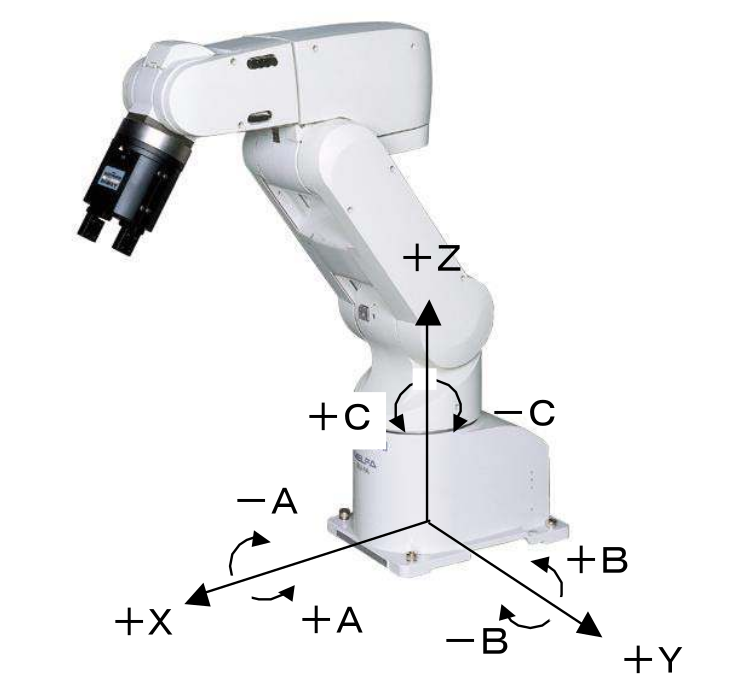
\includegraphics[width=0.6\textwidth]{images/robot_axis.png}
	\caption{Robot coordinate system in XYZ mode}
	\label{fig:robot_axis}
\end{figure}

\begin{center}
	\rowcolors{2}{white}{gray!25}
	\setlength\extrarowheight{4pt}
	\small
	
	\begin{tabularx}{\textwidth}{|p{3cm}|p{4cm}|X|}
		\hline
		\rowcolor{tublau}
		\multicolumn{3}{|c|}{\bf \color{white} \large Gripper}\\
		\hline\hline
		\rowcolor{gray!80}
		\bf MB5-Command & \bf OPC UA & \bf Beschreibung\\
		\hline\hline
		Mov(X,Y,Z,A,B,C) & Move(X,Y,Z,A,B,C): \textbf{ns=4;i=1137} & Modul Roboter (Hand) - Position/Rotation anfahren\\
		HOpen 1 & OpenGripper(): \textbf{ns=4;i=1131} & Modul Roboter (Hand) - Gripper öffnen\\
		HClose 1 & CloseGripper(): \textbf{ns=4;i=1134} & Modul Roboter (Hand) - Gripper schließen\\
		\hline
	\end{tabularx}
\end{center}

\clearpage

\section{System Netzwerk Struktur}
\begin{figure}[!htb]
	\centering
	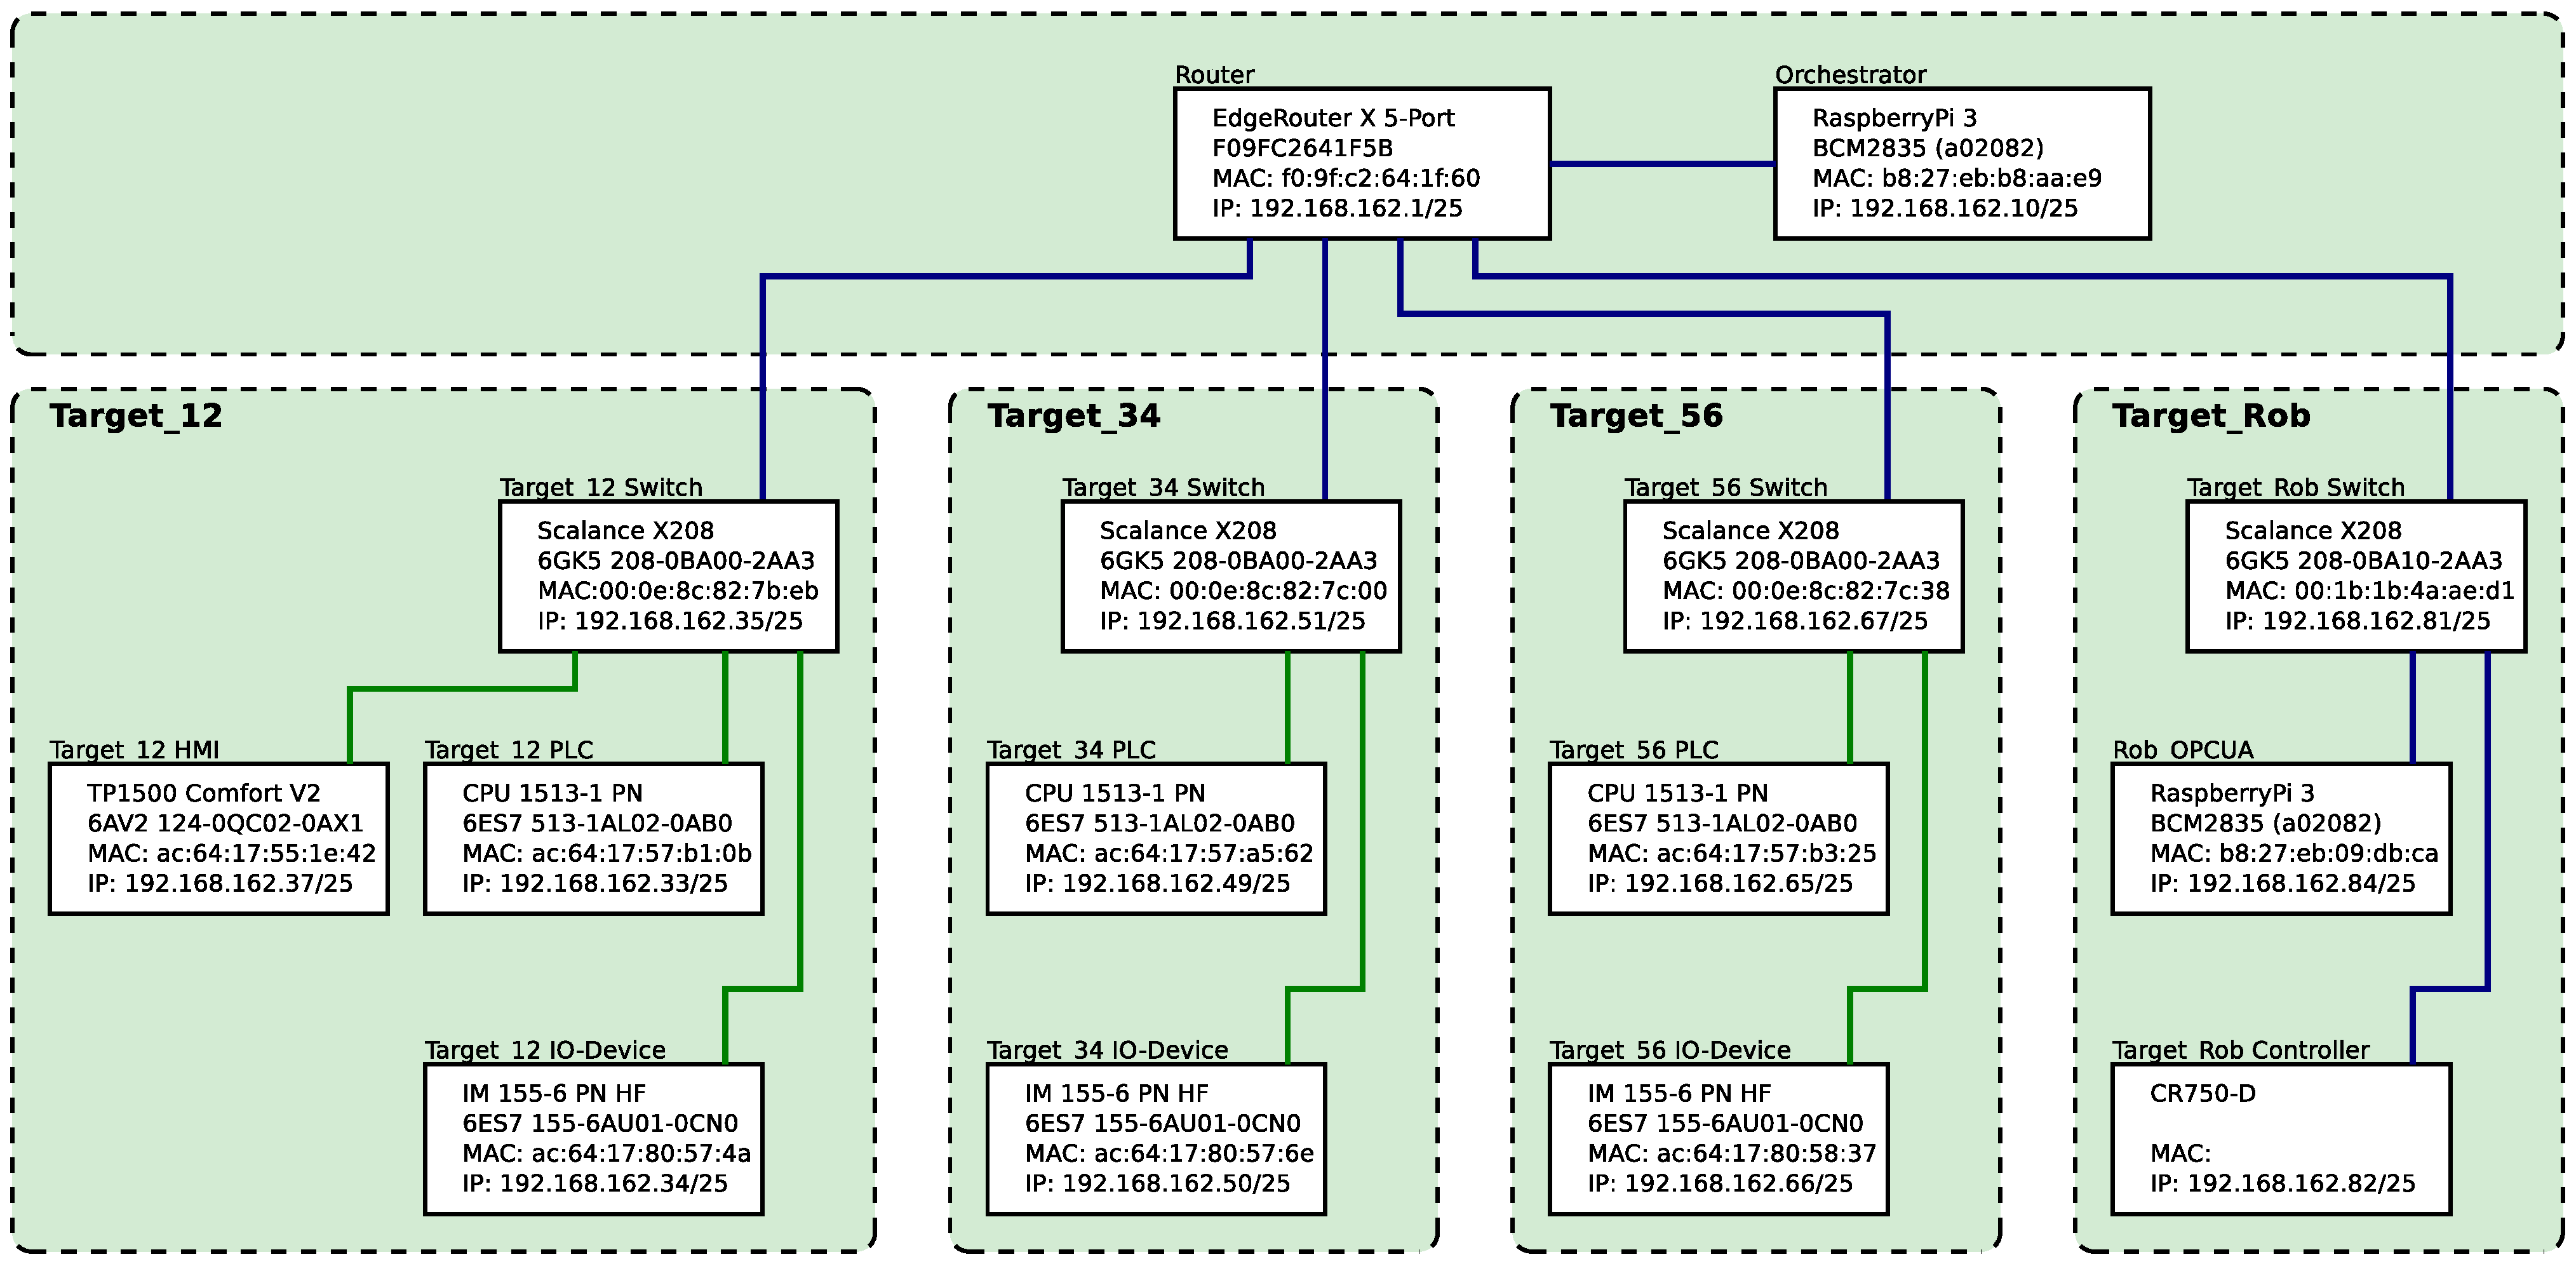
\includegraphics[width=.99\linewidth]{images/Network_Structure}
	\caption{Netzwerk Struktur}
	\label{fig_network_structure}
\end{figure}




\newpage
%\bibliographystyle{plain}
%\bibliography{references}

\makelast

\end{document}
  
